\chapter{Resultados}\label{chap:resultados}

Este capítulo apresenta os resultados experimentais obtidos com o GPT-2
\textit{small} sobre o WikiText-2. A exposição segue a ordem em que os
experimentos foram conduzidos: primeiro as duas estratégias clássicas de poda
--- magnitude (Seção~\ref{sec:res_magnitude}) e estruturada
(Seção~\ref{sec:res_estruturada}) ---, cujos resultados delimitam o problema;
em seguida a estratégia otimizada proposta, em suas duas fases: o
levantamento do perfil de sensibilidade por camada
(Seção~\ref{sec:perfil_sensibilidade}) e a varredura da alocação dele
derivada (Seção~\ref{sec:res_alocacao}). A Seção~\ref{sec:res_sintese}
sintetiza os achados.

\section{Protocolo e Modelo de Referência}\label{sec:res_protocolo}

Todos os experimentos partem do GPT-2 \textit{small} pré-treinado
(124.439.808 parâmetros), avaliado no conjunto de teste do WikiText-2 por
janela deslizante com \textit{stride} de 512 \textit{tokens}. A perplexity do
modelo denso é de \textbf{25,17}, valor coerente com o reportado na
literatura para essa configuração, o que valida a implementação do
procedimento de avaliação. As medições de custo do modelo denso são: 474,70~MB
de memória de parâmetros e 126,6~GFLOPs por janela de 512 \textit{tokens}.

Duas ressalvas metodológicas condicionam a leitura das tabelas que se seguem.

A primeira é que \textbf{todos os resultados deste capítulo são
\textit{one-shot}}: poda-se o modelo pré-treinado e mede-se imediatamente, sem
qualquer \textit{fine-tuning} de recuperação. Essa escolha isola o efeito da
poda do efeito do retreinamento, mas implica que as perplexities aqui
reportadas são substancialmente piores que as da literatura, em que a poda é
seguida de retreinamento. As curvas não devem, portanto, ser lidas como
proposta de configuração de uso, e sim como medida do dano que cada estratégia
de alocação causa por si só.

A segunda é que as varreduras foram executadas em sessões distintas do
ambiente Kaggle, e as medições de \textbf{custo dependem da sessão}. O mesmo
modelo denso registrou 40,5~ms por janela em uma sessão, 54,0~ms em outra e
46,3~ms em uma terceira; o consumo de energia do modelo denso variou de
forma análoga, entre 1176 e 1572~$\mu$Wh. Por essa razão, comparações de tempo
e energia \textbf{entre} varreduras são sempre apresentadas em termos
relativos ao \textit{baseline} da própria sessão, nunca em valores absolutos.
As emissões de $\text{CO}_2$, que dependem adicionalmente do fator de carbono
da rede elétrica do \textit{datacenter} --- que também variou entre sessões
---, não são comparadas entre varreduras.

\section{Poda por Magnitude}\label{sec:res_magnitude}

A Tabela~\ref{tab:magnitude} apresenta a varredura da poda por magnitude
\cite{Han2015} nos dois escopos de alocação implementados:
\textit{global}, em que um único limiar sobre o valor absoluto dos pesos é
aplicado a toda a rede, e \textit{uniforme}, em que cada camada recebe a mesma
fração de poda, com limiar próprio.

\begin{table}[htb]
\centering
\caption{Poda por magnitude \textit{one-shot} no GPT-2 \textit{small} /
WikiText-2. As colunas de custo referem-se ao escopo uniforme; o escopo global
produz valores idênticos, pois nenhum dos dois altera a arquitetura.}
\label{tab:magnitude}
\small
\begin{tabular}{c cc ccc}
\toprule
\textbf{Esparsidade} & \multicolumn{2}{c}{\textbf{Perplexity}} & \multicolumn{3}{c}{\textbf{Custo}} \\
\cmidrule(lr){2-3} \cmidrule(lr){4-6}
 & \textbf{Global} & \textbf{Uniforme} & \textbf{Params. $\neq 0$} & \textbf{Tamanho} & \textbf{FLOPs} \\
\midrule
0\,\%  &    25,17 &    25,17 & 124,4\,M & 474,7\,MB & 126,6\,G \\
10\,\% &    25,40 &    25,47 & 115,9\,M & 474,7\,MB & 126,6\,G \\
20\,\% &    26,87 &    27,22 & 107,5\,M & 474,7\,MB & 126,6\,G \\
30\,\% &    40,23 &    36,42 &  99,0\,M & 474,7\,MB & 126,6\,G \\
40\,\% &   165,20 &   104,82 &  90,5\,M & 474,7\,MB & 126,6\,G \\
50\,\% &  1096,50 &   473,28 &  82,0\,M & 474,7\,MB & 126,6\,G \\
60\,\% &  5121,25 &  2004,20 &  73,5\,M & 474,7\,MB & 126,6\,G \\
70\,\% &  9371,16 &  6891,85 &  65,0\,M & 474,7\,MB & 126,6\,G \\
80\,\% &  8847,27 & 10871,00 &  56,5\,M & 474,7\,MB & 126,6\,G \\
90\,\% &  4612,69 & 13996,88 &  48,0\,M & 474,7\,MB & 126,6\,G \\
\bottomrule
\end{tabular}
\end{table}

O resultado mais importante da tabela está nas três últimas colunas, e é
negativo: \textbf{o custo não cai}. Entre 0\,\% e 90\,\% de esparsidade, o
número de parâmetros não nulos cai de 124,4~M para 48,0~M --- uma redução de
61\,\% ---, enquanto o tamanho em memória, os FLOPs e o tempo de inferência
permanecem rigorosamente constantes. A explicação é direta: a poda não
estruturada substitui pesos por zeros, mas não remove nada da arquitetura. Os
tensores mantêm as mesmas dimensões, e a GPU multiplica os zeros exatamente
como multiplicava os valores originais. O ganho de 61\,\% em parâmetros é
contábil, não físico.

Esse achado responde empiricamente, e pela negativa, à primeira das duas
perguntas que orientam este trabalho --- a de se a redução teórica de
parâmetros se converte em redução real de consumo. Na Tesla T4 utilizada, e
sem suporte de \textit{hardware} ou de \textit{kernels} para esparsidade, a
poda não estruturada não entrega ganho de eficiência algum. A pequena
tendência de queda na energia medida (de 1572 para 1432~$\mu$Wh) é da ordem da
variação observada entre execuções repetidas do mesmo modelo denso e não deve
ser interpretada como efeito da poda.

Quanto à qualidade, a curva de perplexity apresenta um joelho acentuado em
torno de 30\,\%. Até 20\,\% de esparsidade a poda é praticamente gratuita
(acréscimo de 0,3 a 2,1 pontos de perplexity); a partir de 40\,\% a
degradação torna-se explosiva. A região utilizável em regime \textit{one-shot}
é, portanto, limitada a esparsidades de até 20\,\%.

Por fim, a comparação entre os dois escopos revela um cruzamento duplo: os
escopos empatam até 20\,\%, o uniforme domina claramente entre 30\,\% e
70\,\% --- exatamente a faixa em que a escolha de alocação teria consequência
prática --- e o global só apresenta valores menores em 80\,\% e 90\,\%, região
em que ambos os modelos já estão destruídos (perplexity acima de 4600) e a
comparação perde sentido. Na faixa que importa, portanto, a alocação uniforme
é preferível à global. Esse é um resultado contraintuitivo: o escopo global é
o que aloca o orçamento com base em uma medida de importância --- a magnitude
do peso --- e ainda assim perde para a alocação que ignora qualquer medida de
importância. Trata-se do primeiro indício de que a magnitude do peso é um
\textit{proxy} pobre para a importância de um parâmetro.

\section{Poda Estruturada}\label{sec:res_estruturada}

A Tabela~\ref{tab:estruturada} apresenta a varredura da poda estruturada
\cite{Li2017}, adaptada ao \textit{Transformer}: remoção física
de cabeças de atenção e de neurônios das camadas MLP, ordenados por norma
$L_1$. A esparsidade-alvo é expressa como fração de \textit{estruturas}
removidas; a fração de parâmetros efetivamente eliminada aparece como
esparsidade real.

\begin{table}[htb]
\centering
\caption{Poda estruturada \textit{one-shot} (cabeças e neurônios MLP,
escopo global) no GPT-2 \textit{small} / WikiText-2. O tempo de inferência é
normalizado pelo \textit{baseline} da mesma sessão (40,5~ms).}
\label{tab:estruturada}
\small
\begin{tabular}{c c ccccc}
\toprule
\textbf{Estrut.} & \textbf{Perplexity} & \textbf{Params.} & \textbf{Tamanho}
& \textbf{FLOPs} & \textbf{Tempo rel.} & \textbf{Energia rel.} \\
\midrule
0\,\%  &   25,17 & 124,4\,M & 474,7\,MB & 126,6\,G & 1,000 & 1,000 \\
10\,\% &  356,20 & 116,0\,M & 442,6\,MB & 118,0\,G & 0,968 & 0,975 \\
20\,\% & 2102,06 & 107,6\,M & 410,5\,MB & 109,3\,G & 0,908 & 0,945 \\
30\,\% & 2413,52 &  99,0\,M & 377,6\,MB & 100,5\,G & 0,831 & 0,865 \\
40\,\% & 2434,92 &  90,6\,M & 345,5\,MB &  91,9\,G & 0,756 & 0,786 \\
50\,\% & 2402,58 &  81,9\,M & 312,6\,MB &  83,1\,G & 0,688 & 0,714 \\
60\,\% & 2957,26 &  73,5\,M & 280,5\,MB &  74,5\,G & 0,628 & 0,638 \\
70\,\% & 4635,36 &  65,1\,M & 248,3\,MB &  65,9\,G & 0,557 & 0,558 \\
80\,\% & 7620,02 &  56,5\,M & 215,5\,MB &  57,0\,G & 0,503 & 0,489 \\
90\,\% & 5822,89 &  48,1\,M & 183,3\,MB &  48,4\,G & 0,445 & 0,413 \\
\bottomrule
\end{tabular}
\end{table}

O contraste com a Tabela~\ref{tab:magnitude} é o achado central deste
trabalho no plano da eficiência. Aqui \textbf{o custo cai, e cai
proporcionalmente aos parâmetros}: a 90\,\% de estruturas removidas, o tempo
de inferência cai 56\,\%, a energia 59\,\%, o tamanho em memória 61\,\% e os
FLOPs 62\,\%, acompanhando a redução de 61\,\% no número de parâmetros. As
duas tabelas formam, juntas, a resposta completa à primeira pergunta
empírica: a redução de parâmetros só se converte em redução de consumo quando
a poda remove estruturas inteiras da arquitetura, e não quando apenas as
zera.

O preço dessa eficiência, contudo, é severo em regime \textit{one-shot}. Já
com 10\,\% de estruturas removidas a perplexity salta de 25,17 para 356,20 ---
compare-se com 25,40 na poda por magnitude ao mesmo nível. \textbf{Não existe
região gratuita} na poda estruturada sem retreinamento, o que é coerente com o
procedimento original de \citeonline{Li2017}, em que a poda é sempre
seguida de \textit{fine-tuning}.

Dois resultados secundários merecem registro. O primeiro é que a inversão de
escopo observada na magnitude se repete ao contrário: na poda estruturada é o
escopo \textbf{global} que domina, e a alocação uniforme colapsa em taxas
altas (perplexity de 53.313 a 80\,\% e de 827.316 a 90\,\%, contra 7620 e 5823
do global). Somado ao achado da seção anterior, isso estabelece que
\textbf{nenhuma das duas alocações ingênuas vence nos dois regimes} --- a
constatação que motiva diretamente a estratégia otimizada.

O segundo é a assimetria entre os dois tipos de estrutura. Remover cabeças de
atenção é notavelmente mais tolerável que remover neurônios MLP: com 129 das
144 cabeças removidas (90\,\%), a perplexity fica em 781, ao passo que a
remoção equivalente de neurônios MLP produz valores acima de 3900. A curva das
cabeças é, ainda, não monotônica, com mínimo local em torno de 30\,\%
(perplexity 162, inferior aos 237 obtidos com apenas 10\,\% removidas) --- eco
direto do achado de \citeonline{Michel2019} sobre a redundância das
cabeças de atenção. Em contrapartida, as camadas MLP concentram cerca de dois
terços dos parâmetros podáveis, de modo que a poda restrita a cabeças tem
alcance limitado como estratégia de compressão.

\section{Perfil de Sensibilidade por Camada}\label{sec:perfil_sensibilidade}

As duas seções anteriores mostraram que nenhuma alocação ingênua do orçamento
de poda domina o espectro de esparsidade: na poda por magnitude o escopo
uniforme prevaleceu na faixa útil (Seção~\ref{sec:res_magnitude}), enquanto na
poda estruturada foi o escopo global que obteve as melhores perplexidades
(Seção~\ref{sec:res_estruturada}) --- e ambas as alocações colapsam em algum
regime. A hipótese central deste trabalho é que a
causa é comum aos dois casos: as camadas do \textit{Transformer} não são
igualmente importantes, de modo que tanto tratá-las de forma idêntica
(alocação uniforme) quanto confiar exclusivamente na magnitude dos pesos como
proxy de importância (alocação global) distribuem mal o orçamento disponível.

Esta seção reporta o experimento que testa diretamente essa hipótese. Para
cada uma das 12 camadas do GPT-2 \textit{small} e para cada uma das duas
estratégias, poda-se \textbf{apenas} aquela camada a uma taxa-sonda fixa de
50\,\%, mantendo-se as demais intactas, e mede-se a perplexity resultante no
conjunto de teste do WikiText-2. Não há \textit{fine-tuning} --- o
procedimento é \textit{one-shot}, como nas varreduras anteriores. A
degradação é registrada em escala logarítmica,

\begin{equation}\label{eq:delta_log_ppl}
\Delta_{\ell} = \ln\!\left(\frac{\text{PPL}_{\ell}}{\text{PPL}_{\text{base}}}\right),
\end{equation}

\noindent onde $\text{PPL}_{\ell}$ é a perplexity do modelo com apenas a
camada $\ell$ podada e $\text{PPL}_{\text{base}} = 25{,}17$ é a perplexity do
modelo denso. O logaritmo é necessário porque a perplexity de modelos podados
sem recuperação varia por ordens de grandeza: em escala linear, uma única
camada catastrófica tornaria as demais indistinguíveis entre si. O
experimento totaliza 24 medições (12 camadas $\times$ 2 estratégias).

\subsection{Perfil Obtido}\label{subsec:perfil_obtido}

A Tabela~\ref{tab:perfil_sensibilidade} apresenta os resultados e a
Figura~\ref{fig:perfil_sensibilidade} os representa graficamente.

\begin{table}[htb]
\centering
\caption{Perfil de sensibilidade por camada do GPT-2 \textit{small} no
WikiText-2. Cada linha corresponde a podar exclusivamente a camada indicada, à
taxa-sonda de 50\,\%, sem \textit{fine-tuning}. Perplexity do modelo denso:
25,17.}
\label{tab:perfil_sensibilidade}
\small
\begin{tabular}{c cc cc}
\toprule
& \multicolumn{2}{c}{\textbf{Poda por magnitude}} & \multicolumn{2}{c}{\textbf{Poda estruturada}} \\
\cmidrule(lr){2-3} \cmidrule(lr){4-5}
\textbf{Camada} & \textbf{Perplexity} & $\boldsymbol{\Delta_{\ell}}$
                & \textbf{Perplexity} & $\boldsymbol{\Delta_{\ell}}$ \\
\midrule
0  & 37,17 & 0,390 & 1386,43 & 4,009 \\
1  & 26,06 & 0,035 &   27,66 & 0,094 \\
2  & 27,62 & 0,093 &   29,91 & 0,173 \\
3  & 26,28 & 0,043 &   30,23 & 0,183 \\
4  & 30,81 & 0,202 &   31,31 & 0,218 \\
5  & 28,66 & 0,130 &   29,80 & 0,169 \\
6  & 27,09 & 0,074 &   28,90 & 0,138 \\
7  & 26,44 & 0,049 &   28,31 & 0,118 \\
8  & 26,59 & 0,055 &   28,45 & 0,122 \\
9  & 26,76 & 0,061 &   27,63 & 0,093 \\
10 & 26,55 & 0,054 &   28,89 & 0,138 \\
11 & 26,55 & 0,054 &   48,87 & 0,663 \\
\midrule
\textbf{Razão máx./mín.} & \multicolumn{2}{c}{11,3$\times$} & \multicolumn{2}{c}{42,9$\times$} \\
\bottomrule
\end{tabular}
\end{table}

\begin{figure}[htb]
\centering
\caption{Degradação $\Delta_{\ell}$ causada pela poda isolada de cada camada,
à taxa-sonda de 50\,\%. Note-se que as escalas verticais diferem entre os dois
gráficos; na poda estruturada, a barra da camada 0 excede o eixo e está
truncada.}
\label{fig:perfil_sensibilidade}
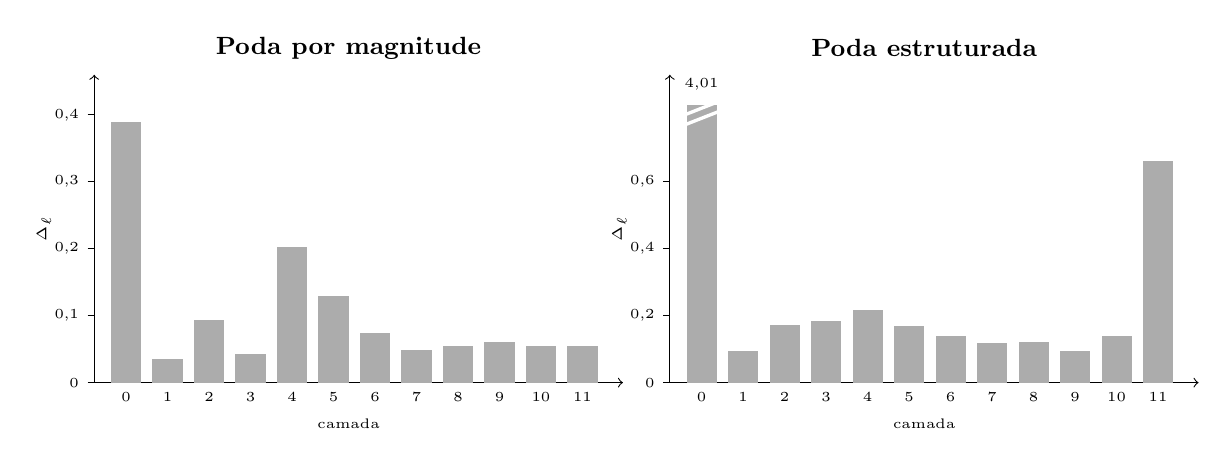
\begin{tikzpicture}[scale=0.85]

  % ---------- painel esquerdo: magnitude ----------
  \begin{scope}
    \draw[->] (-0.2,0) -- (7.7,0);
    \draw[->] (-0.2,0) -- (-0.2,4.6);
    \foreach \y/\lab in {0/0, 1/0{,}1, 2/0{,}2, 3/0{,}3, 4/0{,}4}
      \draw (-0.3,\y*1.0) -- (-0.2,\y*1.0) node[left,xshift=-2pt,font=\tiny] {\lab};
    \foreach \c/\d in {0/0.390, 1/0.035, 2/0.093, 3/0.043, 4/0.202, 5/0.130,
                       6/0.074, 7/0.049, 8/0.055, 9/0.061, 10/0.054, 11/0.054} {
      \fill[gray!65] ({\c*0.62+0.05},0) rectangle ++(0.45,{\d*10});
      \node[font=\tiny] at ({\c*0.62+0.275},-0.22) {\c};
    }
    \node[font=\small\bfseries] at (3.6,5.0) {Poda por magnitude};
    \node[font=\tiny] at (3.6,-0.62) {camada};
    \node[rotate=90,font=\tiny] at (-0.95,2.3) {$\Delta_{\ell}$};
  \end{scope}

  % ---------- painel direito: estruturada ----------
  \begin{scope}[xshift=8.6cm]
    \draw[->] (-0.2,0) -- (7.7,0);
    \draw[->] (-0.2,0) -- (-0.2,4.6);
    \foreach \y/\lab in {0/0, 1/0{,}2, 2/0{,}4, 3/0{,}6}
      \draw (-0.3,\y*1.0) -- (-0.2,\y*1.0) node[left,xshift=-2pt,font=\tiny] {\lab};
    \foreach \c/\d in {1/0.094, 2/0.173, 3/0.183, 4/0.218, 5/0.169,
                       6/0.138, 7/0.118, 8/0.122, 9/0.093, 10/0.138, 11/0.663} {
      \fill[gray!65] ({\c*0.62+0.05},0) rectangle ++(0.45,{\d*5});
      \node[font=\tiny] at ({\c*0.62+0.275},-0.22) {\c};
    }
    % camada 0: barra truncada
    \fill[gray!65] (0.05,0) rectangle (0.50,4.15);
    \draw[white,line width=1.2pt] (0.02,4.0) -- (0.53,4.2);
    \draw[white,line width=1.2pt] (0.02,3.85) -- (0.53,4.05);
    \node[font=\tiny] at (0.275,4.45) {4,01};
    \node[font=\tiny] at (0.275,-0.22) {0};
    \node[font=\small\bfseries] at (3.6,5.0) {Poda estruturada};
    \node[font=\tiny] at (3.6,-0.62) {camada};
    \node[rotate=90,font=\tiny] at (-0.95,2.3) {$\Delta_{\ell}$};
  \end{scope}

\end{tikzpicture}
\fonte{Elaborada pelo autor.}
\end{figure}

O primeiro resultado é que a hipótese se confirma de forma inequívoca: a
sensibilidade está longe de ser uniforme. Sob poda por magnitude, a camada
mais frágil degrada o modelo 11,3 vezes mais que a mais robusta; sob poda
estruturada, 42,9 vezes mais. Tratar as 12 camadas como intercambiáveis ---
que é exatamente o que a alocação uniforme faz --- ignora uma diferença de uma
ordem de grandeza no custo de podar cada uma delas.

\subsection{A Camada 0 como Gargalo}\label{subsec:camada_zero}

O segundo resultado é a magnitude do papel da primeira camada. Nas duas
estratégias ela é a mais sensível, mas o efeito é qualitativamente distinto no
caso estruturado: remover metade das cabeças de atenção e dos neurônios MLP
\textbf{apenas do bloco 0} eleva a perplexity de 25,17 para 1386,43, ou seja,
55 vezes o valor do modelo denso. Para dimensionar esse número, a varredura
estruturada uniforme a 50\,\% --- que poda \textit{todas} as 12 camadas ---
atinge perplexity 4573,00. Em escala logarítmica, a camada 0 sozinha responde
por $4{,}01/5{,}20 \approx 77\,\%$ de toda a degradação produzida pela poda
uniforme do modelo inteiro.

A interpretação é coerente com o papel funcional do primeiro bloco. É nele que
as representações deixam de ser a soma direta de \textit{embeddings} de token
e de posição e passam a ser contextualizadas pela primeira vez; qualquer
informação descartada ali não tem como ser recuperada pelas camadas
subsequentes, que operam sobre um sinal já degradado. Trata-se, portanto, de
um erro que se propaga por toda a pilha, ao contrário de um erro cometido nas
camadas intermediárias.

Na poda estruturada observa-se ainda um segundo ponto crítico na outra
extremidade: a camada 11, imediatamente anterior à cabeça de linguagem,
apresenta $\Delta_{11} = 0{,}663$, quase cinco vezes a mediana das camadas
intermediárias. O perfil estruturado tem, assim, formato aproximado de ``U'':
as bordas da pilha são críticas e o miolo é comparativamente barato. Esse
padrão não se repete na poda por magnitude, cujo perfil decai após um pico
inicial e mantém as últimas camadas entre as mais robustas.

\subsection{Os Perfis Dependem da Estratégia}\label{subsec:perfis_divergem}

O terceiro resultado tem consequência metodológica direta: os dois perfis
\textbf{não} são o mesmo. A correlação de postos de Spearman entre eles é
$\rho = 0{,}50$ --- há concordância, mas parcial. As duas estratégias
coincidem em eleger a camada 0 como a mais crítica e em considerar as camadas
1 e 9 entre as mais robustas, e divergem em praticamente todo o resto: a
camada 11 é a segunda mais sensível sob poda estruturada e apenas a oitava sob
poda por magnitude; a camada 3 é a segunda mais robusta sob magnitude e a
quarta mais sensível sob poda estruturada.

A implicação prática é que não existe um perfil de sensibilidade único do
GPT-2. Sensibilidade é uma propriedade do par (camada, estratégia de poda),
não da camada isoladamente, e o perfil precisa ser levantado separadamente
para cada estratégia --- como foi feito aqui --- sob pena de se alocar o
orçamento com um mapa que pertence a outro método. Esse achado também oferece
uma explicação para a inversão observada nas varreduras ingênuas: como
magnitude de peso e norma de estrutura respondem a aspectos diferentes da
importância de uma camada, é esperado que o escopo global (que decide com base
nessas grandezas) acerte em um caso e erre no outro.

\subsection{Da Sensibilidade à Alocação}\label{subsec:alocacao}

O perfil é um diagnóstico; para virar estratégia, precisa ser convertido em
uma taxa de poda por camada. A regra adotada atribui a cada camada uma taxa
proporcional à sua robustez --- o inverso da degradação medida ---, elevada a
um expoente $\beta$ e escalada por um fator único $\alpha$ tal que a média das
taxas, ponderada pelo número de parâmetros de cada camada, iguale o orçamento
global $s$ pretendido:

\begin{equation}\label{eq:alocacao}
r_{\ell} = \min\!\left(\alpha \cdot \Delta_{\ell}^{-\beta},\ r_{\max}\right),
\qquad
\frac{\sum_{\ell} w_{\ell}\, r_{\ell}}{\sum_{\ell} w_{\ell}} = s,
\end{equation}

\noindent com $w_{\ell}$ o número de parâmetros podáveis da camada $\ell$ e
$r_{\max} = 0{,}95$ um teto que impede que mesmo a camada mais robusta seja
integralmente zerada. O fator $\alpha$ é obtido por bisseção, uma vez que a
fração podada é monótona em $\alpha$. O expoente $\beta$ controla o quanto o
perfil é levado a sério: com $\beta = 0$ a regra degenera na poda uniforme e
com $\beta = 1$ usa-se o inverso puro da degradação; valores intermediários
amortecem a razão entre camadas, o que importa porque essa razão é ilimitada
--- uma camada com $\Delta_{\ell}$ muito próximo de zero receberia
praticamente todo o orçamento.

A Tabela~\ref{tab:alocacao_50} mostra as taxas que a
Equação~\ref{eq:alocacao} produziu para um orçamento global de 50\,\% com
$\beta = 1$. O contraste com a alocação uniforme é acentuado: sob poda
estruturada, a camada 0 recebe 2\,\% de poda e a camada 1 recebe 84\,\%,
enquanto a alocação uniforme aplicaria 50\,\% a ambas.

\begin{table}[htb]
\centering
\caption{Taxas de poda por camada efetivamente aplicadas pela
Equação~\ref{eq:alocacao} para orçamento global de 50\,\% e $\beta = 1$
(coluna \texttt{taxas\_por\_camada} dos registros experimentais). A alocação
uniforme corresponderia a 50\,\% em todas as camadas.}
\label{tab:alocacao_50}
\small
\begin{tabular}{l cccccccccccc}
\toprule
\textbf{Camada} & 0 & 1 & 2 & 3 & 4 & 5 & 6 & 7 & 8 & 9 & 10 & 11 \\
\midrule
Magnitude (\%)   &  8 & 94 & 35 & 75 & 16 & 25 & 44 & 67 & 59 & 53 & 61 & 61 \\
Estruturada (\%) &  2 & 84 & 46 & 43 & 36 & 47 & 57 & 67 & 64 & 85 & 57 & 12 \\
\bottomrule
\end{tabular}
\end{table}

\subsection{Limitações do Perfilamento}\label{subsec:limitacoes_perfil}

Três limitações do procedimento devem ser explicitadas, pois condicionam a
leitura dos resultados da varredura otimizada.

A primeira é que a sonda foi aplicada a uma única taxa (50\,\%). O perfil
mede, portanto, a sensibilidade das camadas naquele regime específico, e nada
garante que a ordenação se mantenha em taxas muito menores ou muito maiores.
A escolha por uma única sonda é uma concessão a custo: cada ponto do perfil
exige uma avaliação completa de perplexity, e o levantamento com múltiplas
sondas multiplicaria proporcionalmente o custo da fase.

A segunda, e mais relevante, é que a sonda mede o efeito de cada camada
\textbf{isoladamente}, ignorando as interações entre elas. Os dados do próprio
experimento mostram que essa aproximação é imperfeita: a soma dos
$\Delta_{\ell}$ individuais sob poda por magnitude é 1,238, ao passo que a
poda uniforme simultânea de todas as camadas a 50\,\% produz degradação
logarítmica de 2,934 --- mais que o dobro. A degradação é fortemente
superaditiva, isto é, os erros introduzidos em camadas distintas se compõem em
vez de simplesmente se somarem. O perfil deve, por isso, ser lido como uma
ordenação relativa de importância, e não como um modelo preditivo da
degradação de uma configuração completa.

A terceira é que todas as medições são \textit{one-shot}, sem
\textit{fine-tuning} de recuperação. Camadas que parecem frágeis nesse regime
poderiam ser recuperáveis com retreinamento, o que eventualmente alteraria a
alocação ótima. A opção pelo regime \textit{one-shot} é deliberada e coerente
com o objetivo do trabalho --- isolar o efeito da poda do efeito do
retreinamento ---, mas restringe a generalidade das conclusões.

Nenhuma dessas limitações invalida o achado principal desta seção, que é
robusto às três: sob qualquer leitura, as camadas do GPT-2 diferem entre si
por mais de uma ordem de grandeza no custo de serem podadas, e essa diferença
é informação que as alocações uniforme e global simplesmente não utilizam. Se
essa informação se converte em ganho efetivo na fronteira entre compressão e
qualidade é o que a varredura da estratégia otimizada, reportada na seção
seguinte, se propõe a verificar.

\section{Varredura da Alocação Guiada por Sensibilidade}\label{sec:res_alocacao}

Esta seção reporta a fase que responde à pergunta central do trabalho: a
alocação derivada do perfil de sensibilidade melhora, de fato, o compromisso
entre compressão e qualidade em relação às alocações ingênuas? As taxas por
camada produzidas pela Equação~\ref{eq:alocacao} foram aplicadas nos mesmos
nove níveis de orçamento das varreduras anteriores, para as duas estratégias, e
avaliadas com o mesmo vetor de métricas. O experimento foi replicado com dois
valores do expoente $\beta$ --- 1,0 e 0,5 ---, o que fornece a ablação da
função de alocação sobre um mesmo perfil.

\subsection{Poda por Magnitude}\label{subsec:aloc_magnitude}

A Tabela~\ref{tab:comp_magnitude} compara as quatro alocações.

\begin{table}[htb]
\centering
\caption{Perplexity da poda por magnitude sob as quatro alocações. Em negrito,
o menor valor de cada linha.}
\label{tab:comp_magnitude}
\small
\begin{tabular}{c cc cc}
\toprule
& \multicolumn{2}{c}{\textbf{Alocação ingênua}} & \multicolumn{2}{c}{\textbf{Guiada por sensibilidade}} \\
\cmidrule(lr){2-3} \cmidrule(lr){4-5}
\textbf{Esparsidade} & \textbf{Global} & \textbf{Uniforme} & $\boldsymbol{\beta = 1{,}0}$ & $\boldsymbol{\beta = 0{,}5}$ \\
\midrule
10\,\% & \textbf{25,40} &    25,47 &    25,44 &    25,44 \\
20\,\% &    26,87 &    27,22 &    26,79 & \textbf{26,57} \\
30\,\% &    40,23 &    36,42 &    34,62 & \textbf{31,20} \\
40\,\% &   165,20 &   104,82 &   193,83 & \textbf{57,30} \\
50\,\% &  1096,50 &   473,28 &  1026,09 & \textbf{447,57} \\
60\,\% &  5121,25 &  2004,20 & \textbf{1524,55} &  2171,79 \\
70\,\% &  9371,16 &  6891,85 & \textbf{1853,30} &  2805,39 \\
80\,\% &  8847,27 & 10871,00 & \textbf{2747,56} &  3715,68 \\
90\,\% & \textbf{4612,69} & 13996,88 & 10398,10 &  7616,63 \\
\bottomrule
\end{tabular}
\end{table}

A alocação guiada vence em oito dos nove níveis, e as margens são
substanciais na faixa de interesse. Em 30\,\% de esparsidade, a perplexity cai
de 36,42 (melhor alocação ingênua) para 31,20 --- uma redução de 14\,\%. Em
40\,\%, o ganho é de 104,82 para 57,30, ou seja, a degradação é praticamente
\textbf{reduzida à metade} usando exatamente o mesmo orçamento de poda. Em
50\,\% a vantagem persiste, ainda que modesta (447,57 contra 473,28). Nos
níveis altos, de 60\,\% a 80\,\%, a configuração com $\beta = 1$ produz
perplexities entre 2,5 e 4 vezes menores que a melhor alocação ingênua ---
embora, nesse regime, todos os modelos já estejam degradados a ponto de a
comparação ter interesse mais teórico que prático.

A única derrota ocorre em 90\,\%, onde o escopo global apresenta o menor valor.
Como discutido na Seção~\ref{sec:res_magnitude}, essa é a região em que a
perplexity de todas as configurações ultrapassa 4600 e a ordenação entre
modelos igualmente inservíveis não carrega significado.

\subsection{Poda Estruturada}\label{subsec:aloc_estruturada}

Na poda estruturada, os ganhos são de outra ordem de grandeza, como mostra a
Tabela~\ref{tab:comp_estruturada}.

\begin{table}[htb]
\centering
\caption{Perplexity da poda estruturada sob as quatro alocações. Em negrito, o
menor valor de cada linha.}
\label{tab:comp_estruturada}
\small
\begin{tabular}{c cc cc}
\toprule
& \multicolumn{2}{c}{\textbf{Alocação ingênua}} & \multicolumn{2}{c}{\textbf{Guiada por sensibilidade}} \\
\cmidrule(lr){2-3} \cmidrule(lr){4-5}
\textbf{Estruturas} & \textbf{Global} & \textbf{Uniforme} & $\boldsymbol{\beta = 1{,}0}$ & $\boldsymbol{\beta = 0{,}5}$ \\
\midrule
10\,\% &   356,20 &    481,13 & \textbf{124,29} &    215,83 \\
20\,\% &  2102,06 &   1484,89 & \textbf{371,07} &    717,19 \\
30\,\% &  2413,52 &   5467,56 & \textbf{724,53} &    923,65 \\
40\,\% &  2434,92 &  10486,71 & \textbf{1301,15} &   9489,87 \\
50\,\% &  2402,58 &   4573,00 & \textbf{2327,59} &   7922,81 \\
60\,\% & \textbf{2957,26} &   5799,76 &  5393,15 &  12322,05 \\
70\,\% & \textbf{4635,36} &  12249,58 & 10130,33 & 103463,60 \\
80\,\% & \textbf{7620,02} &  53313,38 &  8891,77 & 203995,84 \\
90\,\% &  5822,89 & 827316,19 &  5353,85 & \textbf{4830,24} \\
\bottomrule
\end{tabular}
\end{table}

Na faixa de 10\,\% a 50\,\% de estruturas removidas, a alocação guiada com
$\beta = 1$ domina de forma inequívoca. Em 10\,\%, a perplexity cai de 356,20
para 124,29 --- uma redução de 65\,\%. Em 20\,\%, de 1484,89 para 371,07, um
fator de \textbf{quatro}. Em 30\,\%, de 2413,52 para 724,53, um fator de
\textbf{3,3}. Considerando que a Seção~\ref{sec:res_estruturada} concluiu que
não existe região gratuita para a poda estruturada \textit{one-shot}, reduzir a
perplexity a um quarto no mesmo orçamento é o resultado mais expressivo deste
capítulo.

Uma ressalva quantitativa é necessária. Como a remoção de estruturas é
discreta, as taxas fracionárias por camada não são atingíveis exatamente, e a
alocação guiada acaba removendo uma fração de parâmetros ligeiramente menor que
a ingênua no mesmo alvo: em 10\,\%, esparsidade real de 9,20\,\% contra
9,90\,\% do escopo global; em 30\,\%, 29,01\,\% contra 29,95\,\%. Parte da
vantagem observada deve-se, portanto, a um corte marginalmente menor. A
diferença é de menos de um ponto percentual de esparsidade, ao passo que a
diferença de perplexity chega a um fator de quatro, de modo que a explicação
não se sustenta como causa principal --- mas o efeito existe e deve ser
declarado.

A partir de 60\,\%, a ordenação se inverte e o escopo global volta a vencer. A
causa é identificável nas taxas alocadas: a partir desse orçamento, um número
crescente de camadas satura no teto $r_{\max} = 0{,}95$ --- duas camadas em
60\,\%, quatro em 70\,\%, oito em 80\,\% e onze em 90\,\%. Saturadas as
camadas, a alocação deixa de discriminar entre elas e degenera em algo próximo
da poda uniforme sobre o subconjunto saturado, ao mesmo tempo em que concentra
uma pressão crescente sobre as poucas camadas ainda livres. A estratégia
guiada, portanto, \textbf{só é informativa enquanto o orçamento couber dentro
do teto por camada}; acima disso, ela perde sua vantagem estrutural. Esse é um
limite intrínseco de qualquer alocação proporcional com teto, e não um defeito
de implementação.

\subsection{Ablação do Expoente $\beta$}\label{subsec:ablacao_beta}

A comparação entre $\beta = 1{,}0$ e $\beta = 0{,}5$ produz um resultado que
não era antecipado: \textbf{o valor adequado de $\beta$ depende da
estratégia}, e depende dela de forma oposta nas duas.

Na poda estruturada, $\beta = 1$ domina em todos os níveis até 80\,\%, e o
amortecimento é francamente prejudicial --- em 70\,\% e 80\,\% a configuração
com $\beta = 0{,}5$ produz perplexities de 103.463 e 203.996, uma ordem de
grandeza pior que qualquer outra alocação testada. Na poda por magnitude ocorre
o inverso na faixa útil: $\beta = 0{,}5$ é melhor de 20\,\% a 50\,\%, e só a
partir de 60\,\% o expoente pleno passa à frente.

A explicação mais plausível liga-se à dispersão dos perfis. O perfil
estruturado tem razão máximo/mínimo de 42,9$\times$ e é dominado pela camada 0,
cuja fragilidade é tão extrema (Seção~\ref{subsec:camada_zero}) que qualquer
amortecimento da alocação lhe devolve orçamento de poda com consequências
catastróficas: em 70\,\%, $\beta = 0{,}5$ atribui 14,6\,\% de poda à camada 0,
contra 3,0\,\% de $\beta = 1$. Quando o perfil contém um sinal dessa
intensidade, convém segui-lo integralmente. Já o perfil de magnitude tem
dispersão de 11,3$\times$, distribuída entre várias camadas de sensibilidade
intermediária; nele, a razão entre camadas é mais suscetível a ruído de
medição, e amortecê-la funciona como regularização. O expoente $\beta$
comporta-se, assim, como um parâmetro de confiança no perfil: quanto mais
nítido o sinal, maior o $\beta$ que compensa adotar.

\subsection{Efeito sobre o Custo}\label{subsec:aloc_custo}

Do ponto de vista da eficiência, a alocação guiada preserva integralmente o
comportamento da estratégia de base, o que era esperado, uma vez que ela
altera a distribuição do orçamento, não sua natureza. Na poda por magnitude,
tamanho, FLOPs e tempo permanecem constantes, pelo mesmo motivo discutido na
Seção~\ref{sec:res_magnitude}. Na poda estruturada, o custo cai
proporcionalmente: normalizando pelo \textit{baseline} da própria sessão, a
configuração com $\beta = 1$ registra tempo relativo de 0,659 e energia
relativa de 0,674 em 50\,\%, e 0,419 e 0,384 em 90\,\% --- valores
equivalentes, dentro da variação entre sessões, aos 0,688 e 0,714 (50\,\%) e
0,445 e 0,413 (90\,\%) do escopo global.

O achado prático é, portanto, que \textbf{o ganho de qualidade da alocação
guiada é gratuito em termos de custo}: na faixa de 10\,\% a 50\,\% da poda
estruturada, obtém-se uma perplexity de três a quatro vezes menor com
essencialmente o mesmo tempo de inferência, o mesmo consumo de energia e o
mesmo tamanho de modelo. É exatamente o deslocamento da fronteira entre
compressão e qualidade que a segunda pergunta empírica do trabalho se propunha
a investigar.

\section{Síntese dos Resultados}\label{sec:res_sintese}

Os experimentos permitem responder às duas perguntas que orientaram o
trabalho.

À primeira --- se a redução teórica de parâmetros se converte em redução real
de consumo --- a resposta é condicional à granularidade da poda. A poda não
estruturada por magnitude reduz em 61\,\% os parâmetros não nulos sem
alterar em nada o tempo de inferência, a energia, o tamanho em memória ou os
FLOPs: na Tesla T4 utilizada, sem suporte de \textit{hardware} para
esparsidade, o ganho é puramente contábil. A poda estruturada, ao remover
fisicamente cabeças de atenção e neurônios MLP, converte a mesma redução de
61\,\% em parâmetros em quedas de 56\,\% no tempo, 59\,\% na energia e 62\,\%
nos FLOPs. Para o objetivo declarado deste trabalho --- redução do consumo de
energia ---, apenas a poda estruturada é uma estratégia viável.

À segunda --- se a alocação otimizada empurra a fronteira entre compressão e
qualidade --- a resposta é afirmativa, com escopo delimitado. As camadas do
GPT-2 diferem entre si por mais de uma ordem de grandeza no custo de serem
podadas, com a camada 0 respondendo isoladamente por cerca de três quartos da
degradação da poda uniforme; essa informação, que nenhuma alocação ingênua
utiliza, converte-se em ganho mensurável quando incorporada à distribuição do
orçamento. Na poda estruturada --- a estratégia que efetivamente reduz consumo
--- a alocação guiada reduz a perplexity por fatores de três a quatro na faixa
de 10\,\% a 50\,\% de estruturas removidas, sem custo adicional de tempo,
energia ou memória. O escopo da conclusão é delimitado por três fronteiras: o
regime \textit{one-shot}, a saturação da alocação em orçamentos acima de
60\,\%, e o fato de que o perfil de sensibilidade precisa ser levantado
separadamente para cada estratégia de poda, por não ser transferível entre
elas.
